\documentclass[journal]{IEEEtran}
%\usepackage{cite}
\usepackage{graphicx}
\usepackage{epstopdf}
\DeclareGraphicsExtensions{.pdf,.png,.jpg,.eps,.svg}
\usepackage[cmex10]{amsmath}
\usepackage{algorithm}
\usepackage{algorithmic}
\usepackage{longtable}
%\usepackage{array}
%\usepackage{fixltx2e}
%\usepackage{stfloats}
%\usepackage{dblfloatfix}
%\usepackage{url}
% correct bad hyphenation here
\hyphenation{op-tical net-works semi-conduc-tor}
\usepackage{mathchars}
\usepackage{epsfig}
\usepackage{subfigure}
%command
\newcommand{\ipc}{{\sf ipc}}
\newcommand{\Prob}{\bbbp}
\newcommand{\Real}{\bbbr}
\newcommand{\real}{\Real}
\newcommand{\Int}{\bbbz}
\newcommand{\Nat}{\bbbn}
\newcommand{\NN}{{\sf I\kern-0.14emN}}   % Natural numbers
\newcommand{\ZZ}{{\sf Z\kern-0.45emZ}}   % Integers
\newcommand{\QQQ}{{\sf C\kern-0.48emQ}}   % Rational numbers
\newcommand{\RR}{{\sf I\kern-0.14emR}}   % Real numbers
\newcommand{\KK}{{\cal K}}
\newcommand{\OO}{{\cal O}}
\newcommand{\AAA}{{\bf A}}
\newcommand{\HH}{{\bf H}}
\newcommand{\II}{{\bf I}}
\newcommand{\LL}{{\bf L}}
\newcommand{\PP}{{\bf P}}
\newcommand{\PPprime}{{\bf P'}}
\newcommand{\QQ}{{\bf Q}}
\newcommand{\UU}{{\bf U}}
\newcommand{\UUprime}{{\bf U'}}
\newcommand{\zzero}{{\bf 0}}
\newcommand{\ppi}{\mbox{\boldmath $\pi$}}
\newcommand{\aalph}{\mbox{\boldmath $\alpha$}}
\newcommand{\bb}{{\bf b}}
\newcommand{\ee}{{\bf e}}
\newcommand{\mmu}{\mbox{\boldmath $\mu$}}
\newcommand{\vv}{{\bf v}}
\newcommand{\xx}{{\bf x}}
\newcommand{\yy}{{\bf y}}
\newcommand{\zz}{{\bf z}}
\newcommand{\oomeg}{\mbox{\boldmath $\omega$}}
\newcommand{\res}{{\bf res}}
\newcommand{\cchi}{{\mbox{\raisebox{.4ex}{$\chi$}}}}
%\newcommand{\cchi}{{\cal X}}
%\newcommand{\cchi}{\mbox{\Large $\chi$}}

% Logical operators and symbols
\newcommand{\imply}{\Rightarrow}
\newcommand{\bimply}{\Leftrightarrow}
\newcommand{\union}{\cup}
\newcommand{\intersect}{\cap}
\newcommand{\boolor}{\vee}
\newcommand{\booland}{\wedge}
\newcommand{\boolimply}{\imply}
\newcommand{\boolbimply}{\bimply}
\newcommand{\boolnot}{\neg}
\newcommand{\boolsat}{\!\models}
\newcommand{\boolnsat}{\!\not\models}


\newcommand{\op}[1]{\mathrm{#1}}
\newcommand{\s}[1]{\ensuremath{\mathcal #1}}

% Properly styled differentiation and integration operators
\newcommand{\diff}[1]{\mathrm{\frac{d}{d\mathit{#1}}}}
\newcommand{\diffII}[1]{\mathrm{\frac{d^2}{d\mathit{#1}^2}}}
\newcommand{\intg}[4]{\int_{#3}^{#4} #1 \, \mathrm{d}#2}
\newcommand{\intgd}[4]{\int\!\!\!\!\int_{#4} #1 \, \mathrm{d}#2 \, \mathrm{d}#3}

% Large () brackets on different lines of an eqnarray environment
\newcommand{\Leftbrace}[1]{\left(\raisebox{0mm}[#1][#1]{}\right.}
\newcommand{\Rightbrace}[1]{\left.\raisebox{0mm}[#1][#1]{}\right)}

% Funky symobols for footnotes
\newcommand{\symbolfootnote}{\renewcommand{\thefootnote}{\fnsymbol{footnote}}}
% now add \symbolfootnote to the beginning of the document...

\newcommand{\normallinespacing}{\renewcommand{\baselinestretch}{1.5} \normalsize}
\newcommand{\mediumlinespacing}{\renewcommand{\baselinestretch}{1.2} \normalsize}
\newcommand{\narrowlinespacing}{\renewcommand{\baselinestretch}{1.0} \normalsize}
\newcommand{\bump}{\noalign{\vspace*{\doublerulesep}}}
\newcommand{\cell}{\multicolumn{1}{}{}}
\newcommand{\spann}{\mbox{span}}
\newcommand{\diagg}{\mbox{diag}}
\newcommand{\modd}{\mbox{mod}}
\newcommand{\minn}{\mbox{min}}
\newcommand{\andd}{\mbox{and}}
\newcommand{\forr}{\mbox{for}}
\newcommand{\EE}{\mbox{E}}

\newcommand{\deff}{\stackrel{\mathrm{def}}{=}}
\newcommand{\syncc}{~\stackrel{\textstyle \rhd\kern-0.57em\lhd}{\scriptstyle L}~}

\def\coop{\mbox{\large $\rhd\!\!\!\lhd$}}
\newcommand{\sync}[1]{\raisebox{-1.0ex}{$\;\stackrel{\coop}{\scriptscriptstyle
#1}\,$}}

\newtheorem{definition}{Definition}[section]
\newtheorem{theorem}{Theorem}[section]


\newcommand{\fig}[3]{
 \begin{figure*} %[!thb]
 \begin{center}
 \scalebox{#3}{\includegraphics{figs/#1.png}}
 \caption{\label{#1}#2}
 \end{center}
 \end{figure*}
}


\newcommand{\figpdf}[3]{
 \begin{figure*} %[!thb]
 \begin{center}
 \scalebox{#3}{\includegraphics{figs/pdf/#1.pdf}}
 \caption{\label{#1}#2}
 \end{center}
 \end{figure*}
}

\newcommand{\figEPS}[3]{
 \begin{figure*} %[!thb]
 \begin{center}
 \scalebox{#3}{\includegraphics{figs/#1.eps}}
 \caption{\label{#1}#2}
 \end{center}
 \end{figure*}
}


% % % % % % % %


\newcommand{\inp}[1]{\textbf{Input:} #1}
\newcommand{\la}{\leftarrow}


% % % % % % % % %


\begin{document}

\title{ A Many-objective Evolutionary Approach Using Fuzzy Dominance With Bidirectional Bias}

\author{Naheed Anjum Arafat,
		Siddhartha Shankar Das,
        Md.~Monirul~Islam,~\IEEEmembership{Member IEEE}% <-this % stops a space
\IEEEcompsocitemizethanks{
\IEEEcompsocthanksitem Naheed Anjum Arafat is with Bangladesh University of Engineering and Technology, Bangladesh.
\IEEEcompsocthanksitem Siddhartha Shankar Das is with Bangladesh University of Engineering and Technology, Bangladesh.
\IEEEcompsocthanksitem Md. Monirul Islam is with Bangladesh University of Engineering and Technology, Bangladesh.
}
}




% The paper headers
\markboth{IEEE Transactions on Evolutionary Computation}%
{Shell \MakeLowercase{\textit{et al.}}:  A Many-objective Evolutionary Approach Using Fuzzy Dominance With Bidirectional Bias}


% use for special paper notices
%\IEEEspecialpapernotice{(Invited Paper)}


% make the title area
\maketitle

\begin{abstract}
The performance of Pareto dominance based evolutionary algorithms degrades for optimization problems with many objectives (more than 3). This is due to the lack of comparability increasing among the solutions with the increase in number of objectives, since most of the solutions are pareto non-dominated. 

In this paper, we propose a new scalable evolutionary algorithm, called Many Objective Evolutionary Algorithm with Bidirectional Bias (MOEA/BB) for solving many-objective optimization problems. Here, the concept of fuzzy logic is used to define a fuzzy dominance relation which is further used to rank the solutions, thus offering comparability. Also, a novel next generation selection scheme is introduced to mitigate the selection bias inherent in the fuzzy dominance relation. 

Further experiments were conducted to compare the performance of MOEA/BB with four state-of-the-art algorithms in solving eight WFG benchmark problems with 10, 13 and 19 objectives. The experimental results show that, MOEA/BB is able to find better solutions compared to other algorithms in most of the problems.
\end{abstract}

\begin{IEEEkeywords}
pareto dominance, many-objective optimization, fuzzy logic, fuzzy dominance, selection bias, evolutionary algorithms
\end{IEEEkeywords}

% For peer review papers, you can put extra information on the cover
% page as needed:
% \ifCLASSOPTIONpeerreview
% \begin{center} \bfseries EDICS Category: 3-BBND \end{center}
% \fi
%
% For peerreview papers, this IEEEtran command inserts a page break and
% creates the second title. It will be ignored for other modes.
\IEEEpeerreviewmaketitle



\section{INTRODUCTION}
\label{sec:introduction}
\IEEEPARstart{M}{any} real world problems known as Multi-objective Optimization Problems (MOPs) involve multiple objectives to be satisfied concurrently considering several constraints. A pair of objectives may be conflicting or harmonious depending on their underlying correlation \cite{purshouse2003conflict}. If there is a positive correlation between them improving one objective is suffice and we get a single solution meeting the both objectives. If they are conflicting instead of a single solution we get a set of solutions each of which can't be improved in one objective without deteriorating in another. Therefore, we have a set of solutions having trade-off among them  and we say these solutions are non-dominated to one another. Evolutionary algorithms are particularly suitable for MOPs due to the property of achieving the entire set of solution in one single run.

Recently, MOPs of more than three objectives, commonly termed as Many-objective Optimization Problems (MaOPs) \cite{farina2002optimal}\cite{yang2013grid} has taken Evolutionary Multiobjective Optimization (EMO) researchers' attention. Such problems frequently appear in Scientific areas and Engineering and Industrial design; examples may be:

\begin{itemize}
\item Environmental and hydrolic engineering-- \textit{water resource engineering applications} \cite{di2006many}, \textit{water portfolio planning} \cite{kasprzyk2009managing}, \textit{Groundwater pollution remediation} \cite{garrett1999parallel}, \textit{location of site retail and service facilities} \cite{Guimaraes94}

\item Electrical and electronics engineering-- \textit{Synthesis of CMOS Opamp} \cite{zebulum1998synthesis}

\item Telecommunication and network optimization-- \textit{Network Design} \cite{tang1997wireless}, \textit{multicalst flows improve wire-antenna geometries} \cite{donoso2005multi}

\item Robotics and control engineering-- \textit{Fault diagnosis} \cite{marcu1999genetic},  \textit{Controller design}\cite{schroder1997multi}\cite{donha1997genetic}, \textit{Design of controller system} \cite{chipperfield1996multiobjective}\cite{whidborne1995algorithms}\cite{tan1997multi}\cite{duarte2000accelerating}\cite{dakev1995h}, \textit{Robotic manipulation problems} \cite{ortmann2001multi}\cite{coello1998using}

\item Transport Engineering-- \textit{Train system} \cite{laumanns2001multi}\cite{qiu1997prioritising}

\item \textit{Environmental modelling} \cite{jarvis1996towards}

\item Ecology-- \textit{Assessment of ecological models} \cite{reynolds1997multi}\cite{reynolds1997multi}

\item \textit{Process planning} \cite{groppetti1997genetic}\cite{rekiek2006assembly}\cite{rekiek2000dealing}\cite{chen2001multi}, \textit{Time Tabling} \cite{paechter1998timetabling}, \textit{Warehouse management } \cite{poulos2001pareto}

\end{itemize}


MaOPs are particularly challenging to the EMO community due to several reasons.

First, with increase in the number of objectives, increases exponentially the number of solutions required for approximating the entire \textit{Pareto front} (PF). If $n$ points are required for approximating a 1D front, then $n^M$ points are required to approximate an $M$ dimensional front. However, the PF of a $K$-objective optimization problem is a hyper surface of $K-1$ dimension (for bi-objective problems, the PF is a line or curve; for 3-objective problems, the PF is a 2D plane etc. except degenerate surface). Hence for an $M$-objective MOP $n^{M-1}$ points are required for approximating the whole PF. This phenomenon is also known as the \textit{curse of dimensionality} \cite{bellman2003dynamic}.
 
Second, visualization of the objective space is important to a decision maker since in any real world application, a final solution must be chosen from the obtained non-dominated solution set. Several multidimensional visualization techniques have been studied in the MCDM literature \cite{miettinen1999nonlinear}, of which Parallel Coordinate Plot \cite{inselberg1987parallel}\cite{146402} has been used extensively to visualize and interpret PFs interactively. With increasing number of objectives it becomes increasingly difficult to visualize and comprehend the PF. \textit{Many Objective Visualization} is currently a promising research area for application to MOPs.

Third, a considerable number of EMO techniques have been proposed in the last few decades \cite{coello1999comprehensive}. Specially, MOGA \cite{fonseca1993genetic}, NSGA \cite{srinivas1994muiltiobjective}, NSGA-II \cite{deb2002fast},  SPEA \cite{zitzler1999multiobjective}, SPEA2 \cite{zitzler2001spea2} have gained popularity among the researchers. All these algorithms share a common characteristic-- they use either \textit{Pareto dominance based ranking} or \textit{Pareto dominance based counting} as primary selection criteria. However they have been proved to be inefficient for solving MaOPs in a number of studies \cite{purshouse2003evolutionary}\cite{hughes2005evolutionary}\cite{wagner2007pareto}\cite{ishibuchi2008evolutionary}. Even taking large population cannot improve their performance. Attempts have also been made to improve their performance \cite{ishibuchi2008effectiveness}.


Ineffectiveness of Pareto based selection algorithms can be attributed to following reasons:

\begin{itemize}

\item State-of-the-art evolutionary algorithms rely on \textit{Pareto dominance} relation for discriminating good solutions from bad ones. The assigned fitness value of a solution is a function of the number of solutions dominating it and/or the number of solutions dominated by it. The number of non-dominated individuals increases as the number of objectives increases as illustrated in \cite{farina2003fuzzy}. As the number of objectives approaches infinity, the proportion of non-dominated space approaches 1. So, almost all individuals will tend to lie on the non-dominated region and be assigned equal fitness value with respect to \textit{Pareto dominance} based criteria. As a result, popular algorithms will fail to provide strong selection pressure towards the true \textit{Pareto front} of a MaOP.

\item Some algorithms rely on the data structures that grow exponentially in size with increasing number of objectives. For example, in PAES \cite{knowles1999pareto} a map of each grid location (the number of grid location is $r^K$, if there are $K$ objectives each divided into $r$ division) is maintained, indicating amount of solutions residing in each grid location. For higher dimension in order to avoid the \textit{curse of dimensionality}, these algorithms are forced to divide each objective into lower number of divisions. More solutions lie in the same grid. As a result, diversity suffers, although convergence increases.

\item Some algorithms which rely on fixed size archive like PAES or SPEA happen to loss some solutions which might have dominated \textit{archived solutions} at a later generation. This phenomenon is termed as \textit{fitness deterioration} by Hanne \cite{hanne1999convergence}.


\end{itemize}

Keeping the poor scalability of the state-of-the-art algorithms in mind, the primary objective is to devise an algorithm for solving MaOPs. Here, we assume, in high dimension almost all of the solutions are non-dominated. In light of this assumption, we can simplify three basic characteristics of our algorithm:

\begin{itemize}
\item The approximation set provided by the algorithm must be as close to the \textit{Pareto front} as possible.
\item The solutions in the approximation set must be distributed uniformly and as sparse as possible in the objective space.
\item We assume no intervention from \textit{Decision Maker} i.e. the algorithm assumes a posteriori approach to solving an MOP. So, the algorithm does not strive towards any particular preferred portion of the frontier or \textit{region of interest} (ROI), rather it is expected to approximate the entire \textit{Pareto front}.
\end{itemize}

The remainder of the paper is organized as follows. In Section \ref{sec:litrev}, an in-short background of the multi-objective optimization and fuzzy sets is reviewed. Afterwards, a detailed description of the proposed algorithm along with differences in working procedure with other existing algorithms are given in Section \ref{sec:ourapproach}. In Section \ref{sec:expstudies}, we discuss the benchmark problems and performance measures used in our experimental studies. The performance of the proposed approach and its comparison with other algorithms are also demonstrated. Finally, some concluding remarks and an outlook to implied future works are presented in Section \ref{sec:conclusion}.


\section{LITERATURE REVIEW}
\label{sec:litrev}

\subsection{Multi-Objective Optimization:}
A MOP including $m$ kinds of objective function is defined as follows:
\begin{center}
Minimize/Maximize $y = f(x) = (f_1(x), f_2(x),\dots,f_m(x))$\\
Subject to $x \in F$
\end{center}

\indent Where $x$ is a vector of decision variables i.e. the decision vector, $F$ is the decision space, $f:F \rightarrow \real^m$ consists of m real valued objective functions, $y$ is called the objective vector and $\real^m$ is called the $m$--dimensional objective space. If $x \in \real^n,$ all the objectives are continuous and $F$ is described by 
\begin{center}
$F = \{x \in \real^n\mid h_j(x)\leq 0, j=1,2,\dots,k \}$
\end{center}
where $h_j$ are continuous constraint functions and $n$ is the number of decision variable.

Solving a MOP is to determine from among the set $F$ of all members-- a particular subset $F^* = {x^{*}_1, x^{*}_2,\dots,x^{*}_n}$ which yields optimum values (minimum/maximum) for all the objective functions.

\begin{definition} (Pareto Dominance) :
Considering minimization problem, suppose $f(u),f(v)\in \real^m$. $u$ is said to dominate $v$ if and only if $f_i(u)\leq f_i(v)$ for every $i\in {1,\dots, m}$ and $f_j(u)<f_j(v)$ for at least one $j \in {1,\dots,m}$. Mathematically, 

\begin{center}$\forall i \in M : f_i(u) \leq f_i(y) \cap \exists j\in M : f_j(u)<f_j(v).$\end{center}

where $M = {1, 2,\dots,m}$.
When $u$ dominates $v$, we denote $f(u) \succeq f(v)$. Pareto dominance is irreflexive, transitive and anti-symmetric. 
\end{definition}


\begin{definition} (Pareto-optimality) :
We say that a decision vector $x^*\in F$ is \textit{Pareto-optimal} w.r.t $F$ if it is dominated by no other $x$ in $F$. $f(x)$ is called a \textit{Pareto-optimal vector}. In other words, there exists no feasible decision vector $x\in F$ which would improve some objective without causing simultaneous decrease in at least one other objective. The set of all such \textit{Pareto-optimal} points is called \textit{Pareto-optimal Set} (PS) and the set of all such \textit{Pareto-optimal vectors} is the \textit{Pareto-optimal Front} (PF) \cite{miettinen1999nonlinear}.
\end{definition}

\begin{definition} (Ideal vector and Nadir vector) :
An objective vector $z^{ideal} = (z^{ideal}_1, \dots, z^{ideal}_m)$ constructed using the best values of objective functions in the complete Pareto-optimal front $PF^{*}$ is called an ideal objective vector. 
On Contrary, Nadir vector is the vector $z^{nadir} = (z^{nadir}_1,\dots,z^{nadir}_m)$ constructed using the worst values of the complete Pareto-optimal front. Hence, for minimization problems, we have $z^{ideal}_i = \min_{x \in PF} f_i(x)$ and  $z^{nadir}_i = \max_{x \in PF} f_i(x)$
\end{definition}

\subsection{Fuzzy-Sets}

Fuzzy sets were first introduced by Lotfi Zadeh \cite{zadeh1965fuzzy} as extensions to classical set theory. Instead of binary membership to a set (i.e. belongs to or not belongs to), fuzzy set allows partial membership denoted by a real number between 0 and 1.
Formally, a fuzzy set is a tuple $(A,\lambda_A)$ where $A$ is a set and $\lambda_A: A \rightarrow [0, 1]$. For each $x\in A, \lambda_A(x)$ is the degree of member of $x$ in $A,x \in (A, \lambda_A) \leftrightarrow x \in A \wedge \lambda_A(x)\neq 0$.


\subsection{Existing Approaches}
It is hard to classify approaches devised by EMO researchers to handle many-objective optimization problems since the term `many-objective optimization' coined by Farina in 2002 \cite{farina2002optimal}. A diverse set of algorithms exist in the literature.\\

\textit{Modified pareto dominance approaches:} The problem of incomparability among the solutions led the researchers to modify pareto dominance relation in order to offer comparibility. Some distinguished works are--- dominance area control \cite{sato2007controlling}, k-optimality \cite{farina2002optimal}, fuzzy pareto dominance \cite{koppen2005fuzzy}, $\epsilon$-dominance \cite{laumanns2002combining}, pareto cone-dominance \cite{batista2011comparison}, pareto $\alpha$-dominance \cite{batista2011comparison}. Experiment shows that modified pareto dominance relations offer better convergence than pareto dominance.\\

\textit{Non-dominated ranking:}
Ranking Non-dominated solutions so that they can be further differentiated is not a new concept. Drechsler et al. \cite{drechsler2001multi} proposed relation \textit{favour} which considers the number of objectives in which a solution is better than another as primary selection criteria. It was further modified to consider the amount of betterment in \cite{sulflow2007robust}. A set of non-dominated solutions are ranked according to each separate objective and assigned a fitness value as an aggregate function of individual ranks in each objectives in \cite{kukkonen2007ranking}--termed as `ranking dominance'. Other ranking schemes include `winning score' \cite{maneeratana2006compressed}, di Pierro's $k$-optimality \cite{di2006many}. Knowles made a comparative study on different non-dominated ranking approaches in \cite{corne2007techniques} and results indicated that `average ranking' performs better. In \cite{ishibuchi2008effectiveness} they showed that although convergence of NSGA-II increases, diversity suffers. Similar conclusion was drawn in \cite{kukkonen2007ranking}.\\

\textit{Indicator based approaches:}
Indicator based performance metric has been used to measure the quality of non-dominated solution sets for long \cite{knowles2002metrics}\cite{zitzler2003performance}\cite{okabe2003critical}. The hypervolume space covered by the non-dominated set, first used as performance measure in \cite{zitzler1998multiobjective} has been incorporated in an evolutionary algorithm-- IBEA(Indicator Based Evolutionary algorithm) by Zitzler et al. \cite{zitzler2004indicator}. Wagner et al. \cite{wagner2007pareto} reported good result by IBEA for many-objective problems. The prime concern for IBEA is its large computation overhead incurred by hypervolume calculation. Bader and Zitzler devised an algorithm-- HypE \cite{bader2011hype}  for faster approximate hypervolume calculation based on Monte-carlo sampling, thus mitigating the computational burden. Recently, WFG devised by While et al. \cite{while2012fast} calculates exact hypervolume much faster for more than 5 objectives – although the worst case complexity is still exponential ($O(2^n)$ where n = total number of solutions). Another algorithm for S-metric calculation- HOY has worst case time complexity of $O(n^{M/2}*log n)$ where M = number of objectives and n = number of solutions. What makes hypervolume based EA's so popular is that hypervolume has the inherent property of representing convergence and diversity. A non-dominated set with better convergence and better diversity than another non-dominated set will always have hypervolume greater than the other.\\

\textit{Objective reduction:}
Dimensionality reduction is another method for inducing preference ordering over the points in a solution set. Not all pair of objectives are conflicting. Correlation may exists among them. Hence, if a many-objective problem can be reduced to a 2 or 3 objective instance keeping the problem characteristic intact, we can apply existing algorithms on them. This thought has led to approaches based on objective reduction. Deb and Saxena \cite{deb2005finding} proposed a principal component based (PCA) NSGA-II procedure which iteratively reduces objectives at each generation and then apply NSGA-II. PCA based NSGA-II performs better when a many-objective problem could be reduced to 2 or 3 objective. However if all the objectives of an $M$ objective problem are conflicting, objective reduction is not possible and the approach is amenable to degraded performance. Brockhoff et al. \cite{brockhoff2009objective}\cite{brockhoff2006all} discussed under which condition objective minimization is possible, generalized the notion of conflicting objectives, redundant objectives and minimal objective set and proposed both exact algorithm and heuristic to determine the minimal objective set while preserving the dominance structure of the problem. The main problem of these approaches is their underlying assumption that objectives can be reduced. For many real world problems this assumption is not true.\\

\textit{Aggregation based approaches/Scalarizing function based approaches:}
These are non-pareto based EA. These approaches convert the set of objectives $(f_1,f_2,f_3,\dots,f_n)$ into a single objective $(F)$ by expressing $F$ as a weighted sum or weighted Tchebycheff of objectives $(f_1,f_2,f_3,\dots,f_n)$. And instead of minimizing these objectives, we minimize $F=(\sum w_j*f_j)$ --thus converting the many-objective problem into a single objective optimization problem. The main advantage of this approach is that it eliminates the need for exponential increase of non-dominated solution with increasing number of objectives. Also it is easier to calculate the weighted sum of objectives rather than computing the hypervolume. The main drawback of this approach is to determine a good set of weights since, it grows with the number of objectives. A number of algorithms has been proposed-- MSOPS \cite{hughes2003multiple}, MSOPS-II \cite{hughes2007msops}, MOEA/D \cite{zhang2007moea}.\\

\textit{Co-evolutionary approaches:}
Preference information i.e Decision makers priority can offer comparability among non-dominated solutions. Some preference based approaches include \cite{fleming2005many}\cite{deb2006reference}\cite{thiele2007preference}. Preference information can also be incorporated as a set of goal vectors. Co-evolving the set of solutions with the set of goal vectors is another way of solving many-objective optimization problems. One realization of this approach is PICEA-g \cite{wang2013preference} where solutions will try to dominate goals and goals will try to be non-dominated by the solutions and their individual fitness is proportional to their individual criteria. Co-evolutionary approaches has been long used for solving MOP's. A comprehensive study can be found in \cite{kleeman2006coevolutionary}. The potential of co-evolutionary approaches in solving many-objective optimization problems, first demonstrated in \cite{purshouse2011preference}, is still underrated and considered by the authors as a new avenue for exploration.\\

\textit{Fuzzy based approaches:}
Pareto dominance doesn't incorporate the degree of dominance in its optimality criteria. A solution will either be dominated (dominating) or non-dominated w.r.t another solution and another one will either be dominating (dominated) or non-dominated w.r.t the other. Farina and Amato \cite{farina2004fuzzy} proposed \textit{fuzzy optimality} where a solution can be dominated/dominating and non-dominated to a certain degree. Fuzzy membership function are used to fuzzify the difference of objective values in each objective and the degree of dominance of one solution over another is the sum of degree of dominance in individual objectives. Nasir et al. \cite{5949696} suggested a new MOEA based on Decomposition with fuzzy dominance concept (MOEA/DFD) to compare two solutions and used the scalar decomposition method of MOEA/D only when one of the solutions fails to dominate the other in terms of a fuzzy dominance level. Koppen et al. \cite{koppen2003fuzzy} studied the fuzzification of the Pareto dominance relation to yield the degree of dominance between two solutions. The degree of dominance is calculated between each pair of solutions and each solution is assigned a ranking value (FPD ranking) within this set as the maximum of the all pair degree of mutual dominances. Hence, if a solution is dominated by at least one solution it will give a rank value of $1$. Lowest rank individuals are considered best individuals. Based on this, an extension of the standard genetic algorithm, fuzzy-dominance-driven GA (FDD-GA), was proposed. In \cite{koppen2005fuzzy} it was demonstrated that FPD ranking resolves the problem of missing dominated points in higher dimension. Among recent approaches Zhenan et al. \cite{he2012new}\cite{he2014fuzzy} proposed a new fuzzy based dominance and applied it in NSGA-II and SPEA2 instead of pareto dominance. Experimental result shows that it achieves better convergence and diversity than MOEA/D \cite{zhang2007moea}, NSGA-II \cite{deb2002fast}, SPEA2 \cite{zitzler2001spea2}, FDD-GA \cite{koppen2003fuzzy} and other fuzzy based approaches. Rachmawati et al. \cite{rachmawati2010incorporation} integrated decision makers preference as a set of imprecise goal vectors each of which may be defined with any of three degree of precision: small, medium and large.\\

\textit{Other approaches:}
A \textit{Grid based Evolutionary algorithm (GrEA)} has been proposed by Yang et al. \cite{yang2013grid} where a user defined parameter (\textit{div}) is used to partition the objective space between lowest and highest value in each objective into grid. Each solution has an associated \textit{grid coordinate} and \textit{grid dominance} (defined in terms of grid coordinate of two solutions) is used to offer comparability among the solutions. Grid Crowding distance (GCD), Grid ranking (GR) and Grid Coordinate point distance (GCPD) are taken into account while selecting the best individual. GCD ensures diversity and GR and GCPD ensures convergence. The basic drawback of this method is that its performance is sensitive to \textit{div} parameter. If number of partition in each objective \textit{(div)} is smaller, convergence suffers. For larger value of \textit{div}, diversity suffers. 


\section{A MANY-OBJECTIVE EVOLUTIONARY APPROACH USING FUZZY DOMINANCE WITH BIDIRECTIONAL BIAS (MOEA/BB)}
\label{sec:ourapproach}

\subsection{Motivation}
The main issue regarding a MaOP is the lack of comparability among the solutions. Regarding this issue a fuzzy comparability mechanism is introduced which can classify otherwise incomparable solutions. The provided comparability is responsible for bias of the solutions towards different directions. Now, instead of letting bias take its own accord, a controlled mechanism is used. During fitness assignment in each generation, it is possible to forcefully bias the solutions towards targeted directions while keeping progress towards PF. Combining each such biased approach together ensures diversity among the solutions while keeping convergence towards PF.


\subsection{Background Knowledge of Fuzzy Logic}

We take the \textit{fuzzification} of \textit{Pareto dominance} approach to solve MaOPs. As discussed before, in conventional \textit{Pareto dominance}, a solution can be \textit{dominated} or \textit{dominating} or \textit{non-dominated}. However objective difference between a pair of solutions can also be interpreted as element of fuzzy set. A solution may dominate or be dominated by another solution by a certain degree simultaneously. For example, $(1,10),(3,5)$ are \textit{Pareto non-dominated}, even if they are \textit{non-dominated}, we say, $(3,5)$ is better than $(1,10)$ in a degree because $(3,5)$ is 2 worse than $(1,10)$ in the $1^{st}$ objective and 5 better in $2^{nd}$ objective considering minimization problem. The degree of goodness in $2^{nd}$ objective excels the degree of badness in $1^{st}$ objective. To measure this degree of goodness or badness we need \textit{membership function}.

In this study, we define the \textit{membership function} for each objective based on \textit{Sigmoid membership function} $(F_g)$ which is adaptive, means depending on the distribution of the value of the solutions in each objective it adapts its parameters for that objective. A \textit{Sigmoid membership function} for an objective is shown in Fig. \ref{sigmoid}:

%\figEPS{sigmoid}{A simple Sigmoid Membership Function}{0.5}

\begin{figure}[!t]
\centering
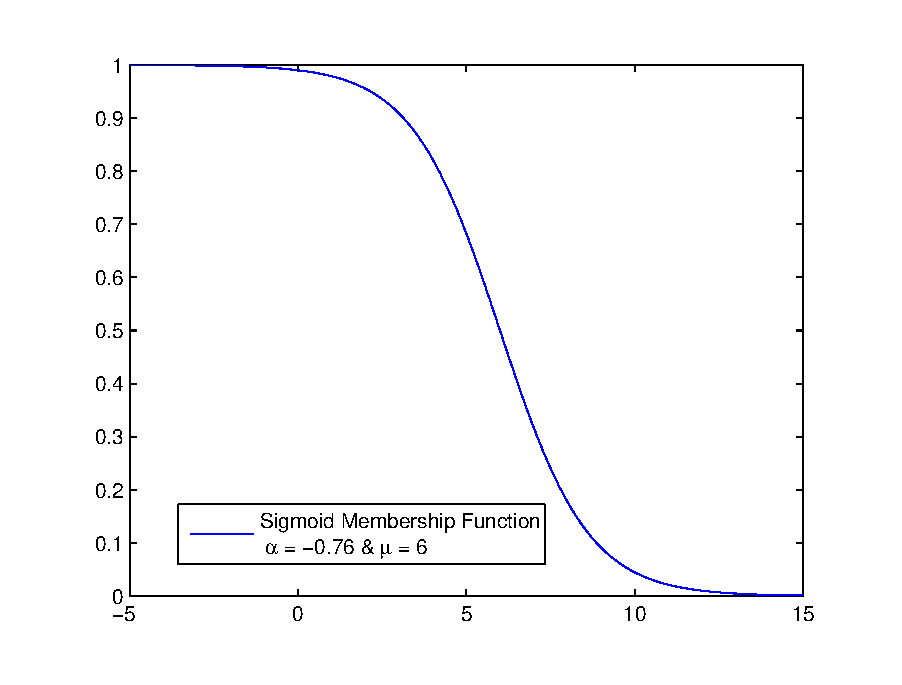
\includegraphics[width=2.5in]{figs/sigmoid.eps}

\caption{A simple \textit{Sigmoid Membership Function} with $\alpha = -0.76$ \& $\mu = 6$ }
\label{sigmoid}
\end{figure}


\begin{equation}\label{eqn:sigmoidEqn} 
F_g(x)=A +\frac{(K-A)}{1+e^{\alpha(x-\mu)}}
\end{equation}

Where $A$ is the \textit{lower-asymptote} which is $0$ for our case. $(K-A)$ set to $1$ which is the  \textit{upper-asymptote}. Hence, the output value will be bounded by $1$ to $0$.
Here $\mu$ is the value where maximum growth occurs and $\alpha$ is the growth rate. Therefore,
\begin{equation}F_g(x)=\frac{1}{1+e^{\alpha(x-\mu)}}\end{equation}
Each objective has a \textit{membership function} of this type. These \textit{Sigmoid membership functions} are then applied in the definition of \textit{fuzzy dominance} relation.\\
Since, dominance in each objective has been defined as a fuzzy set, they can be easily combined. Two basic operators are frequently used in fuzzy logic literature - fuzzy \textit{`and'} operator or \textit{t-norms} and fuzzy \textit{`or'} operator or \textit{s-norms}. There are several \textit{t-norm} and \textit{s-norm} operators in fuzzy logic literature. A comprehensive study on them can be found in \cite{zimmermann1992fuzzy}.\\
\textit{Algebric product (as t-norm)} and \textit{Algebric sum (as s-norm)} deserves special attention. They are defined as follows:\\
\textit{Algebric product} = \begin{math}\{(x,\mu_A(x)*\mu_B(x))\mid x\in X\}\end{math}\\
\textit{Algebric sum} = \begin{math}\{(x,\mu_A(x)+\mu_B(x)-\mu_A(x)*\mu_B(x))\mid x\in X\}\end{math}\\
The intersection or Algebric product of \textit{fuzzy dominance} values in each objective indicates how much a solution dominates another.


\subsection{Fuzzy dominance Relation}

Consider two objective vectors, $u(u_1,u_2,\cdots,u_k)$ and $v(v_1,v_2,\cdots,v_k)$ for a $k$-objective minimization problem.

We define $d_{u,v}^{i}=u_i-v_i$ where $i=1,2,3,\dots,k$. $dom_{u,v}^{i}=F_g(d_{u,v}^{i})$ represents the fuzzy dominance degree of $u$ over $v$ in $i^{th}$ objective.

Fuzzy \textit{t-norm} operator is used to combine the fuzzy values, $\phi_{u,v}=\prod\limits_{i=1}^{k} dom_{u,v}^{i}$ which indicates how much $u$ fuzzy dominates $v$.

Similarly, $\phi_{v,u}=\prod\limits_{i=1}^{k} dom_{v,u}^{i}$ indicates how much $v$ fuzzy dominates $u$.

We say, $u$ dominates $v$ $(u \succeq_F v)$ iff $\phi_{u,v} > \phi_{v,u}$ and $u$ and $v$ are non-dominated if $\phi_{u,v}$ = $\phi_{v,u}$. Fuzzy dominance relation is irreflexive, asymmetric like Pareto dominance relation but unlike Pareto dominance it is non-transitive. Non-transitivity is particularly useful in solving MaOPs because it doesn't impose a total ordering over the solution set.

The following example explains how fuzzy domination works in conjunction with these \textit{membership functions}.\\
Initially, $\phi_{u,v}=1$ and $\phi_{v,u}=1$. It means solution $u$ completely dominates solution $v$ and solution $v$ completely dominates solution $u$. At this stage they are fuzzy non-dominated.
Normalization rule is defined for the two solutions as\\
$\phi_{u,v}^{Norm}=\frac{\phi_{u,v}}{\phi_{u,v}+\phi_{v,u}}$ and
$\phi_{v,u}^{Norm}=\frac{\phi_{v,u}}{\phi_{u,v}+\phi_{v,u}}$\\
Therefore, normalization at this stage results, $\phi_{u,v}^{Norm}=0.5$ and $\phi_{v,u}^{Norm}=0.5$.

Now, consider for $i^{th}$ objective $u_i<v_i$. $x=u_i-v_i <0$ and $y \rightarrow 1$. Therefore, $dom_{u,v}^{i}$ will be still close to $1$ i.e. $u$ still dominates $v$ completely.
On contrary, $x=v_i-u_i>0$ and depending on the magnitude, $y$ is within $1$ and $0$. $x$ – for other pair of solutions is $\bar{x}$, on average. Now, the smaller $x$ is relative to $\bar{x}$, the closer $y$ will be to $1$. Similarly, the larger $x$ is relative to $\bar{x}$, the closer $y$ will be to $0$. So, $dom_{v,u}^{i}$ will still be between $1$ and $0$. It indicates how much $v$ dominates $u$ in $i^{th}$ objective.\\
Say, $y = 0.5$, means $dom_{v,u}^{i}=0.5$. Since, $dom_{u,v}^{i}=1$ and $dom_{v,u}^{i}=0.5$, it indicates $u$ dominates $v$ in $i^{th}$ objective.

Again, say, for $j^{th}$ objective $u_j>v_j$. $y = 0.5$ means $dom_{v,u}^{j}=0.5$.
Since, $dom_{u,v}^{j}=0.2$ and $dom_{v,u}^{j}=1$, we say, $v$ dominates $u$ in $j^{th}$ objective.\\
After inspecting these 2 objective,
$\phi_{u,v} = 1\times dom_{u,v}^{i} \times dom_{u,v}^{j} = 1\times 1 \times 0.2 = 0.2$ and 
$\phi_{v,u} = 1\times dom_{v,u}^{i} \times dom_{v,u}^{j} = 1\times 0.5 \times 1 = 0.5$.

We say, $v$ fuzzy dominates $u$ in $i$ and $j$ objectives altogether. This concept can be further extended to any number of objectives. According to the normalization rule defined earlier, $\phi_{u,v}^{Norm} = 0.28$ and $\phi_{v,u}^{Norm} = 0.72$. Therefore, we say, $u$ dominates $v$ by degree $0.28$ and $v$ dominates $u$ by degree $0.72$, although they are \textit{Pareto non-dominated}. A simple algorithmic procedure is shown in Algorithm \ref{alg:fuzzydominanceAlgo}.

\begin{algorithm}[!h]
\textbf{Input:} Two input solutions $u$ and $v$\\
\textsc{Fizzy dominates}
\begin{algorithmic}[1]
 \STATE $\phi_{u,v}=1$
 \STATE $\phi_{v,u}=1$
 \FOR{$i=1$ \TO $m$ } 
 \STATE{Compute $dom_{u,v}^{i}$ and $dom_{v,u}^{i}$}
 \STATE{$\phi_{u,v}=\phi_{u,v}\times dom_{u,v}^{i}$} 
 \STATE{$\phi_{v,u}=\phi_{v,u}\times dom_{v,u}^{i}$} 
 \ENDFOR
\end{algorithmic}
\caption{Fuzzy Domination}
\textbf{Output:} How much $u$ dominates $v$ and $v$ dominates $u$
\label{alg:fuzzydominanceAlgo}
\end{algorithm}

\subsection{Adaptive definition of membership functions}

The \textit{membership function} is used to fuzzify the difference of two solutions in a particular objective. Now instead of defining a fixed parameter \textit{membership function} for all objectives (in that case function parameters will be problem dependent), we define different \textit{membership function} for different objectives. The parameters of each \textit{membership function} are dependent on the distribution of the solutions in that particular objective.

The \textit{membership function} determines how much one solution dominates another with respect to all such dominations for a particular objective. Different pair of solutions produce different dominance degree and the shape of the function depends on its distribution.

For estimating parameters of the \textit{membership function} for a particular objective, absolute differences of solution value for that objective has been taken for all distinct pair solutions. %This value is taken once as same value will be found if the difference was computed for the other solution perspective.

To estimate $\alpha$ (growth rate) and $\mu$ (point of maximum growth) the \textit{membership function} is defined in such a way that it gives value $0.5$ when $x$ $(d_{u,v}^i)$ is equal to the average difference. If their difference is close to average difference of such pair of solutions, we say they dominate each other by degree $0.5$.

Therefore, $\mu$ = average of all pair difference in a particular objective.

For a particular objective, the distribution of a set of objective values can be skewed in any side like left, middle or right depending on their mean. Therefore, objective differences can also be skewed to a side. $\alpha$ has been defined such that at $(\mu-2\sigma)$ the output value returns $0.99$. If we set $0.99$ at the minimum difference and $0.01$ at maximum difference then it could be biased towards a single difference.

Defining $\alpha$ in this way reduces the sensitivity to extreme standalone objective values. The reason behind choosing \textit{Sigmoid function} as the \textit{membership function} is: non-linearity of this function helps differentiate among the most common differences which are likely to lie between the range $(\mu \pm 2\sigma)$.

The mean and variance are numerically computed by Knuth's running mean and running variance estimation algorithm \cite{Knuth:1997:ACP:270146} which is $O(n)$. Therefore, the overall performance of the algorithm doesn't degrade.\\

\subsection{Ranking based on fuzzy dominance}
Assuming there are $n$ individuals in the competition pool, every individual is paired with other $n-1$ individuals respectively, forming $n-1$ pairs of competition. For individual $u$, in each of $n-1$ pairs, it is compared with the other individual $v$ using fuzzy-dominance relation and both $\phi_{u,v}$ (How much $u$ dominates $v$) and $\phi_{v,u}$ (How much $v$ dominates $u$). Then, fuzzy product value is normalized as $\frac{\phi_{v,u}}{\phi_{u,v}+\phi_{v,u}}$,which represents domination performance of $v$ with respect to $u$. After calculating each pair, all performance values of the amount by which $v$ dominates are summed together to obtain a sum value. This sum value is then divided by $(n-1)$ and the divided value is regarded as the fitness value that is used for ranking the solutions.
Solutions are then sorted into ascending order by the fitness value. So the first solution in the sorted order is considered as the best solution in terms of being the least dominated by others. The ranking procedure is shown in Algorithm \ref{alg:rankingProcessAlgo}.


\begin{algorithm}[!h]
\textbf{Input}: A competition pool containing $n$ individuals\\
\textsc{Ranking}
\begin{algorithmic}[1]
\FOR{$i=1$ \TO $n$ } 
\STATE{$S_i=0$} \COMMENT{calculate sum value of point solution $i$}
\STATE{\FOR{$j=1$ \TO $n$ }
		\STATE{$p=\frac{\phi_{j,i}}{\phi_{i,j}+\phi_{j,i}}$} 
		\COMMENT{calculate performance value of $i$ with $j, j \neq i$}
		\STATE{$S_i=S_i+p$} 
	   \ENDFOR} 
\STATE{$S_i=\frac{S_i}{n-1}$} 	   
\ENDFOR
\STATE{Sort Individuals by the $S$ value in ascending order.}
\end{algorithmic}
\caption{Ranking Process}
\textbf{Output:} Solutions sorted in ascending order by how much they are dominated by others.
\label{alg:rankingProcessAlgo}
\end{algorithm}


\subsection{Next Generation Selection Scheme}

%Suppose, there is a pool of $2n$ solutions and $n$ solutions are selected for next generation.If  
%One choice might be: after assigning the fitness value and sorting them into rank, taking the best $n$ solutions from the list. This approach ensures convergence. However, diversity is affected, because the solutions will be biased towards one direction of the objective space in the long run. Solutions will be biased towards cornered solution in case of concave surface and biased toward centered solution for convex surface. The reason behind this lies in the process of defining membership function, fuzzy dominance and rank assignment.

%\textbf{Figure has to be given showing how solutions are biased}

Our selection scheme is divided into two strategy: In one, we keep the convergence of the solutions while keeping their diversity biased towards outer extremes and in another we keep the convergence of the solutions while keeping their diversity biased inwards. So combining this two approach we can maintain the diversity while converging towards the entire \textit{Pareto front}.

Consider A pool of $2n$ non-dominated solutions from which $n$ solutions have to be selected as next generation.

The next generation is taken in two sweeps. In the first sweep, $(n+d)$ solutions are selected from $2n$ solutions. After that, $n$ solutions out of these $(n+d)$ solutions are selected. Here $d$ is chosen heuristically. Typically $d$ is $n/4$. To select $(n+d)$ solutions in first sweep, we scan through the sorted ranked list of solutions where solutions are sorted in ascending order of the degree by which they are dominated.
Two crowding distance comparators have been defined. One will sort the solutions based on crowding distance in descending order from high value to low value, while keeping corner solutions (solutions whose crowding distances are infinity) in the last of the sorted list i.e. giving them the least priority. We call this comparator \textit{CDCornerPointMinPriority}. The another one will sort them in descending order while keeping those solutions with infinite crowding distances (extreme solutions) in the first positions in the sorted list. In other words, this operator termed as \textit{CDCornerPointMaxPriority} gives the most priority to the corner solutions. Therefore, the selection bias of the two comparators are in two different directions.

\textit{For inward tendency}, consider $m$ number of objectives and we maintain a list of solutions (\textit{Takensolutionlist}) of  initial size $0$. Scanning process is continued until half-way of non-dominated solution set (\textit{S}), considering $2m$ solutions at a time. $\lceil m/2\rceil$ best solutions selected according to \textit{CDCornerPointMinPriority} comparator are added to $Takensolutionlist$ and discarded from $S$ simultaneously. The whole process is continued until the number of taken solutions becomes $(n+d)$.

The selection of $m/2$ solutions from $2m$ solutions is done by first assigning crowding distance to the $2m$ solutions. Solutions are then sorted by \textit{CDCornerPointMinPriority} and we take first $m/2$ solutions from the sorted list.
Now in this method we take the required $(n+d)$ solutions during the first sweep. Then for selecting the $n$ solutions among them, we reassign \textit{crowding distance} value among them and sort them using \textit{CDCornerPointMinPriority} so that any crowded solution that may be taken into first sweep are eliminated from final solution set. And we also give least priority to the border solutions. The reason is twofold- first, it has been experimented that giving least priority to the border extreme solutions helps keep diversity in many objective problem. Second, it also helps keep the bias inward.

Here we ignore the solutions that resides in the corner, instead we take solutions that have greater crowding distance but don't reside in the corner. Now as the scanning length is half of solution list length, multiple scans will be needed and solutions are taken mostly from the front of the ranking list. So the convergences of solutions are ensured. At the same time, each time taking solutions in this manner keeps the bias to the inwards. Algorithm \ref{alg:inwardBiasAlgo} show how the procedure works.


%\figpdf{Drawing1}{Inwards biased selection scheme}{0.7}

\begin{algorithm}[!h]
\textbf{Input:} Nondominated Solution Set $(S)$ ranked by their degree of being dominated by others, The number of solutions required to be selected from this solution set $(N)$\\
\textsc{Selection Scheme I}
\begin{algorithmic}[1]
\STATE{$Extra= size(S)- N$}
\STATE{$Takensolutionlist=\emptyset$}
\STATE{$TakeInFirstSweep=N+Extra/4$} \COMMENT{$(n+d)$}
\STATE{$maxTake=\lceil m/2\rceil$}
\WHILE{$size(Takensolutionlist) < TakeInFirstSweep$} 
	\STATE{$left=0$}
	\STATE{$right=2m$}
	\STATE{$k=\lceil size(S)/2 \rceil$}
	\FOR{$i=left$ \TO $k$ }
		\STATE{Reassign Crowding Distance to the solutions from $s[left]$ to $s[max(right,size(S))]$}
		\STATE{$Localbest$ = $maxTake$ number of population taken from $s[left]$ to $s[max(right,size(S))]$ according to \textit{CDCornerPointMinPriority}}
		\STATE{$Takensolutionlist=Takensolutionlist \union Localbest$}
		\STATE{$left=right$}
		\STATE{$right+=2m$}
	\ENDFOR
\STATE{$S=S \setminus Takensolutionlist$}	
\ENDWHILE
\STATE{Sort the solutions taken on first sweep by \textit{CDCornerPointMinPriority} and take the required $N$ population from the sorted solution set.}
\end{algorithmic}
\textbf{Output}: $N$ population with inward tendency.
\caption{Selection Scheme with Inward Bias}
\label{alg:inwardBiasAlgo}
\end{algorithm}


\textit{For outward tendency},
Consider again the number of objectives $m$, and we maintain a list of solutions, \textit{Takensolutionlist} of  initial size $0$. Scanning process is done until the end of Nondominated Solution Set (\textit{S}), considering $2m$ solutions at a time. $m$ best solutions selected according to the \textit{CDCornerPointMaxPriority} are added to $Takensolutionlist$ and discarded from $S$ simultaneously. Sweeping over the nondominated set (S) in this way is continued until the number of taken solution taken become $(n+d)$.

The selection of $m$ best solutions is done by first assigning \textit{crowding distance} between the $2m$ solutions. Then they are sorted using comparator \textit{CDCornerPointMaxPriority} and first $m$ of them are selected. So for an $m$ objective problem it will select the corner solutions among the first $2m$ solutions.

Note that selecting among the first $2m$ in ranked gives priority to convergence. And while taking the $m$ solutions in this manner from the $2m$ means we give priority to outward solutions locally.Now in this method we take the required $(n+d)$ solutions during the first sweep.

In second sweep, in order to select $n$ solutions from $n+d$ solutions, we reassign \textit{crowding distance} value among them and sort them using \textit{CDCornerPointMaxPriority} so that any adjacent solutions that may be taken in first sweep are eliminated and solutions are biased outwards. Algorithm \ref{alg:outwardBiasAlgo} shows how the procedure works.


%\figpdf{Drawing2}{Outward biased selection scheme}{0.7}

\begin{algorithm}[!h]
\textbf{Input:} Nondominated Solution Set $(S)$ ranked by their degree of being dominated by others, The number of solutions required to be selected from this solution set $(N)$\\
\textsc{Selection scheme II}
\begin{algorithmic}[1]
\STATE{$Extra= size(S)- N$}
\STATE{$Takensolutionlist=\emptyset$}
\STATE{$TakeInFirstSweep=N+Extra/4$} \COMMENT{$(n+d)$}
\STATE{$maxTake=m$}
\WHILE{$size(Takensolutionlist) < TakeInFirstSweep$} 
	\STATE{$left=0$}
	\STATE{$right=2m$}
	\STATE{$k=size(S)$}
	\FOR{$i=left$ \TO $k$ }
		\STATE{Reassign Crowding Distance to the solutions from $s[left]$ to $s[max(right,size(S))]$}
		\STATE{$Localbest$ = $maxTake$ number of solutions taken from $s[left]$ to $s[max(right,size(S))]$ according to \textit{CDCornerPointMaxPriority}}
		\STATE{$Takensolutionlist= Takensolutionlist \union Localbest$}
		\STATE{$left=right$}
		\STATE{$right+=2m$}
	\ENDFOR
\STATE{$S=S \setminus Takensolutionlist$}	
\ENDWHILE
\STATE{Sort the solutions taken on first sweep by \textit{CDCornerPointMaxPriority} Take the required $N$ population from the sorted solution set.}
\end{algorithmic}
\textbf{Output}: $N$ solutions with outward tendency.
\caption{Selection Scheme with Outward Bias}
\label{alg:outwardBiasAlgo}
\end{algorithm}


Combining these two approaches we can keep offspring generation tendency outward and inward while keeping the convergence. Therefore, ultimately it will keep the diversity among the solutions while maintaining selection pressure towards the \textit{Pareto-optimal front}.\\

The pseudocode for the proposed MOEA/BB algorithm is presented in Algorithm \ref{alg:moeabbalgo}

\begin{algorithm}[!h]
\textbf{Input:} population size ($N$); max. generation ($G$); search space\\
\textsc{Main Loop of MOEA/BB}
\begin{algorithmic}[1]
\STATE{Initialize populations randomly. Generation count, $t=0$.}
\STATE{A parent population $P_t$ is used to create mating pool. Parents selected using Binary Tournament are recombined and mutated to create a child population $Q_t$ of size $N$.}
\STATE{$R_t = P_t \union Q_t$. The population $R_t$ will have size $2N$.}
\STATE{Compute the parameters of Sigmoid membership function for each objective.}
\STATE{Rank the solutions using fuzzy dominance.}
\STATE{Next generation is selected using bidirectional bias. Next generation population $\left| {P_{t+1}} \right|  = N$ is selected using inward bias in even generations and using outward bias in odd generations.}
\STATE{$P_{t+1}$ is used as next generation parent. The process is continued from Step 2 until $t$ reaches max. generation, $G$.}
\end{algorithmic}
\textbf{Output}: Non-dominated solutions at generation $T_G$.
\caption{Many Objective Evolutionary Algorithm with Bidirectional Bias}
\label{alg:moeabbalgo}
\end{algorithm}


\section{Difference with other work}

There are some non-trivial differences between the proposed method and other fuzzy-based approaches. Farina and amato \cite{farina2004fuzzy} compared solutions based on the number of objectives and degree of betterment in each objective. Three fuzzy sets are defined and three membership functions are defined to quantify them: better than,worse than and equal. Two types of membership function (linear and Gaussian) has been advised to use and DM will specify their parameters according to domain knowledge. \textit{t-norm} and \textit{t-conorms} are applied in optimality criteria. Nasir et al. \cite{5949696} calculated fuzzy dominance level between two solution by passing their objective difference to an exponential membership function and using product operator to combine them. Zhenan et al. \cite{he2014fuzzy} used left \textit{Gaussian membership function} to fuzzify the objective differences. Fuzzy product operator is used and a problem-dependent heuristically chosen threshold value is used to rank the solutions. NSGA-II is used as baseline algorithm. 

Our approach is different due to the following reasons-

\begin{itemize}
\item All fuzzy based approaches share a common property – they somehow fuzzify the objective differences and combine those values using some operator. Our approach is not an exception. But none of them considered that different objective might have different trade-off magnitude. As a result, the magnitude might not be same and their differences might not follow the same distribution. Using the same membership function to fuzzify them would fail to offer proper comparability between two solutions. For example, consider the  of objective values for 3 solution in ~{Table~I} (range of each objective is shown in brackets).


\begin{table*}%[!thb]
\begin{center}
\caption{Solution Values}
\begin{tabular}{| c | c | c | c | c | c | c |}
\hline
&\textbf{Obj1 [1, 5]} & \textbf{Obj2 [5, 30]} & \textbf{Obj3 [5, 30]} & \textbf{Obj4 [5, 35]} & \textbf{Obj5 [5, 45]} & \textbf{Obj6 [5, 55]}\\
\hline

Solution1 & 1 & 15 & 25 & 35 & 45 & 55 \\
\hline

Solution2 & 5 & 5 & 5 & 5 & 5 & 5 \\
\hline

Solution3 & 5 & 30 & 30 & 5 & 5 & 5 \\
\hline

\end{tabular}
\end{center}
\label{table_spiderplot}
\end{table*}

%\figpdf{spiderplot}{Differentiability of 3 Nondominated Solutions}{.6}
%\fig{spiderplot}{Differentiability of 3 Nondominated Solutions}{.2}

\begin{figure}[!t]
\centering
\scalebox{.3}{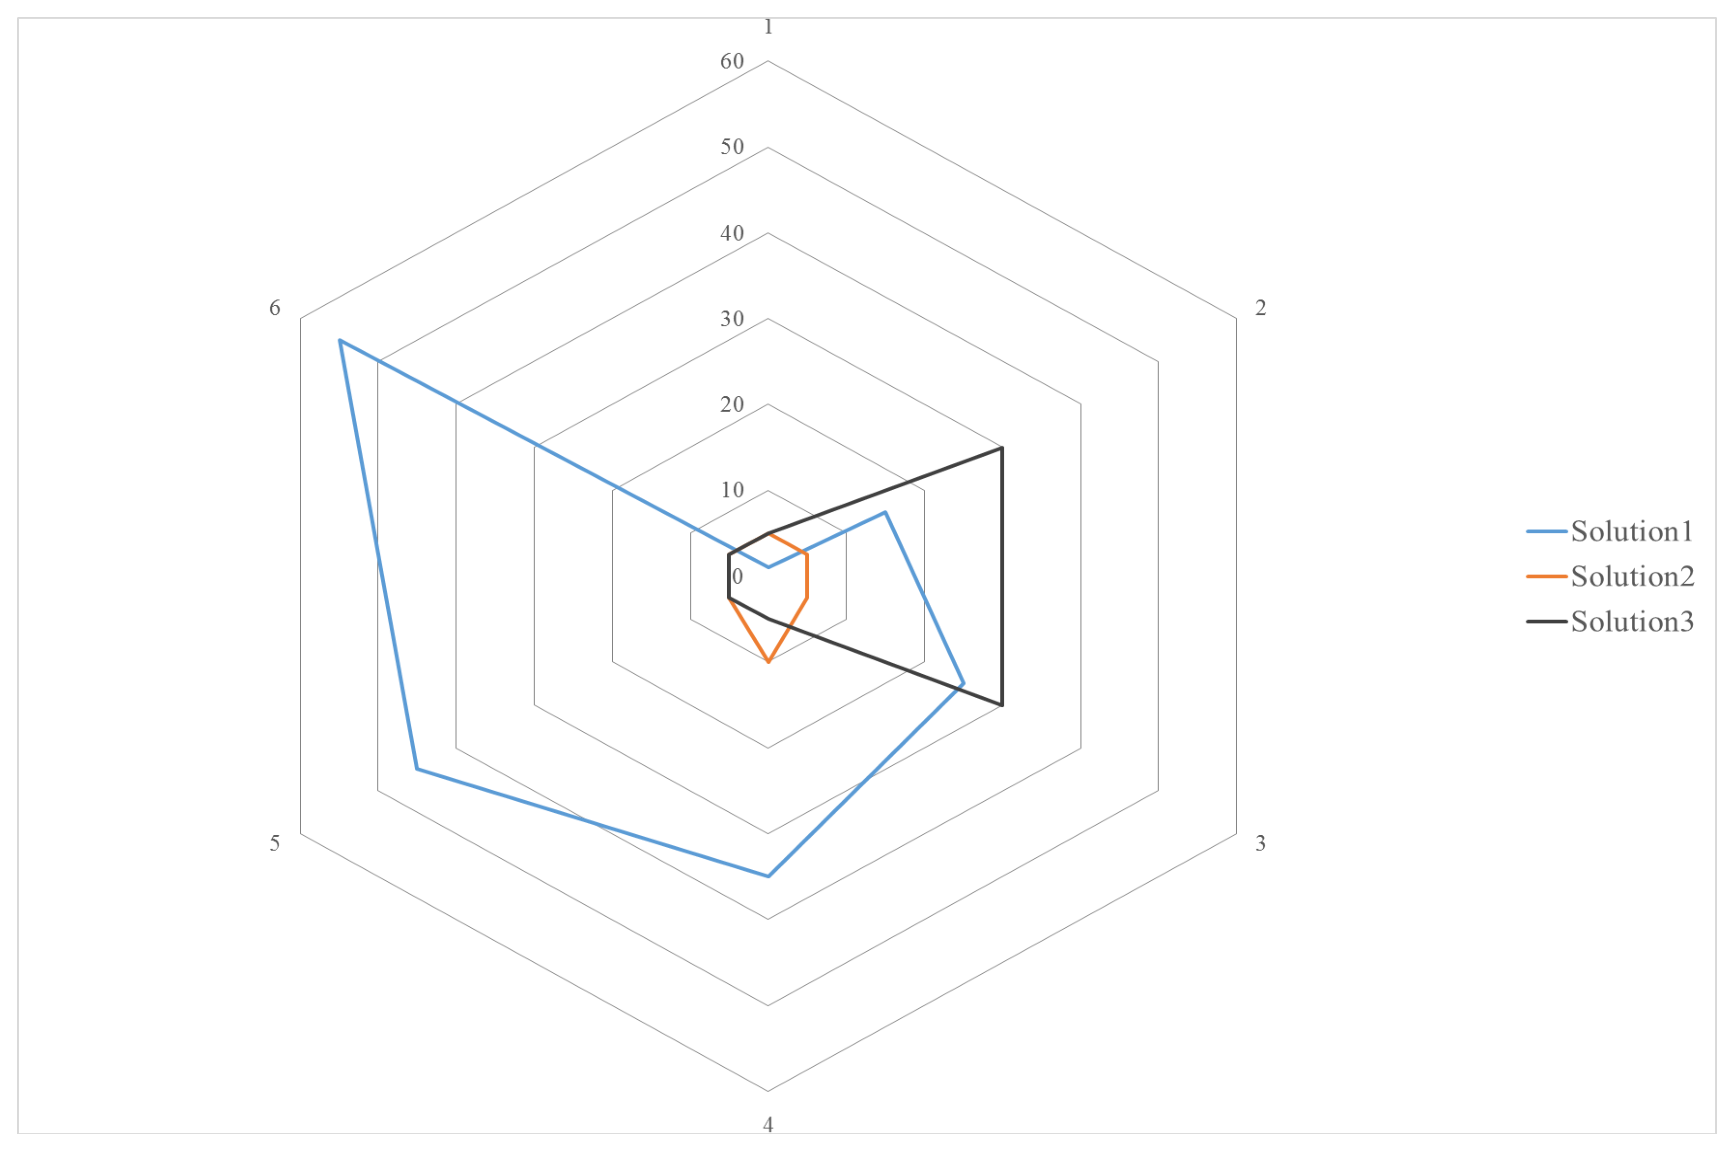
\includegraphics{figs/spiderplot.eps}}
\caption{Differentiability of 3 Nondominated Solutions}
\label{spiderplot}
\end{figure}


\textit{Solution2} is better than \textit{Solution1} in 1 objective, whereas \textit{solution3} is better in 3 objectives as shown in Fig. \ref{spiderplot}. If membership function is defined in $[1,5]$ range (if difference tends to 5, fuzzy value tends to 1). As 1 is the asymptote of the membership function, for difference value beyond 5 fuzzy value increases very slowly. As a result, $\phi_{2,1}$ will be very little different from $\phi_{3,1}$ which naturally shouldn't be.


\item Although only fuzzifying Pareto relation would help converge the solutions which is the prime issue for Many-objective problems, still there remains a separate unresolved issue- diversity. Therefore, a separate diversity maintenance scheme is required. Nasir et al. \cite{5949696} used MOEA with decomposition, Zhenan et al. \cite{he2014fuzzy} used NSGA-II as the baseline algorithm. There is no diversity maintenance mechanism in FDD-GA in \cite{koppen2003fuzzy} by Koppen et al. We used prioritized crowding distance scheme for maintaining diversity. Since, only sampling solutions with high crowding distance and high rank might maintain high density around corners and low density around middle of the Pareto front.
\end{itemize}

\section{EXPERIMENTAL STUDIES}
\label{sec:expstudies}

To understand the efficacy of our algorithm we have to compare it with several MOEA on existing benchmark problem suits. Although many algorithms require special parameter settings, some generic EA parameter settings remains the same.

\subsection{Selected MOEAs for Comparison}
We have selected PICEA-g \cite{wang2013preference}, GDE3 \cite{kukkonen2005gde3}, HypE \cite{bader2011hype}, MOEA/D \cite{zhang2007moea} as the competitors of our algorithm. PICEA-g has been selected because it is one of the latest algorithms which has shown promising results on several many-objective scalable benchmark problem suits. GDE3 is an improved version of differential evolution based evolutionary algorithm GDE \cite{lampinen2001s}. HypE and MOEA/D have been selected as contenders from indicator based and aggregation based evolutionary approaches. Both of them have proved their worthiness in solving MaOPs in their respective areas.

\subsection{Benchmark Problems}

WFG toolkit \cite{huband2006review} is the benchmark problem suit for our experimental studies. WFG2-WFG9 have been used in our study. WFG test suit has been chosen because all WFG problems are scalable to high dimension with the following additional features –
\begin{itemize}
\item No extremal or medial parameters.
\item Have known pareto optimal sets i.e known analytic solution.
\item Scalable number of parameters.
\item Dissimilar tradeoff ranges i.e. different objective values has different domain magnitude.
\item Have no constraints.
\end{itemize}
WFG2 is convex, WFG3 is linear and others have a concave pareto front. In terms of separability, only WFG4, WFG5 and WFG7 are separable. WFG2 is disconnected and WFG3 is degenerate. In terms of modality only WFG2, WFG4 and WFG9 are multimodal i.e. they have multiple local optima. WFG5 and WFG9 are deceptive making the global optima in an unlikely place. WFG2, WFG3, WFG6, WFG7, WFG8 are unimodal. 

\subsection{Performance Metrics}

\textit{Generational Distance (GD)}: 
The concept of generational distance (GD) was defined by Veldhuizen and Lamont (1998) as a way of estimating how far is $PF_{true}$ (true/actual pareto front) from $PF_{obtain}$, (obtained final non-dominated set) and is defined as: 
$GD= \sqrt{(\sum\limits_{i=1}^{n}) d_i^2}$

Where n is the \textit{cardinality} of $PF_{obtain}$ and $d_i$ is the \textit{Euclidean phenotypic distance} between each of these and the nearest member of $PF_{true}$. $GD = 0$ indicates that all the solutions are on the \textit{true pareto front}. Lower value of $GD$ means better convergence.\\

\textit{Inverted Generational Distance (IGD)}:
Another convergence metric. But distance is measured with respect to $PF_{true}$ i.e how far the $PF_{obtain}$ is from $PF_{true}$. Hence,
$IGD=\frac{\sqrt{(\sum\limits_{i=1}^{n}d_i^2)}}{n}$

Here, $n$ is the cardinality of $PF_{true}$ and $d_i$ is the \textit{Euclidean phenotypic distance} between each of these and the nearest member of $PF_{obtain}$. In case, $PF_{obtain}$ has few points and clustered together $GD$ value will be small but $IGD$ will still be large.\\

\textit{Space Uniformity}:
Suppose, $d_1,d_2,\dots,d_n$ are defined as follows:
$d_i = min ( D_{i,j} | i\neq j)$
here, $D_{ij}$ means \textit{manhattan distance} between solution $i$ and solution $j$. Space uniformity is the standard deviation of $d_1,d_2,\dots,d_n$.\\
%\textit{Spread}:
%Spacing doesn't take into account the extent of spread. Hence,even if, the solutions are not near the pareto front, uniformly distributed solutions in the objective space will give lower value of space uniformity. To solve this problem, Deb et al. \cite{deb2002fast}suggested Spread metric which is defined as follows:
%\begin{equation}
%\delta = \frac{\sum\limits_{m=1}^{M}d_m^e+ \sum\limits_{i=1}^{|Q|-1}d_i-\bar{d}}{\sum\limits_{m=1}^{M}d_m^e+(|Q|-1)\bar{d}}
%\end{equation}
%Here, $d_i$ = \textit{manhattan distance/Euclidian distance} between $i^{th}$ and $(i+1)^{th}$ solution (assuming $PF_{obtain}$ is sorted)$d_m^e$ is the distance between the extreme points of sorted $PF_{true}$ and $PF_{obtain}$.
%$|Q|$ is the \textit{cardinality} of $PF_{obtain}$.

\textit{HyperVolume(HV)}:
For an m-dimensional objective space \textit{HyperVolume} is the volume bounded by the \textit{nadir vector} and $PF_{obtain}$ in Euclidean $m$ space.\\

\textit{HyperVolume Ratio (HVR)}:
Suppose,$H_1$ be the \textit{HyperVolume} of the non-dominated set $PF_{obtain}$ and $H_2$ be the HyperVolume of $PF_{true}$. $HR$ is defined as $\frac{H_1}{H_2}$. $HR$ will always be in the interval $[0,1]$.

To measure convergence in our study Generational Distance (GD) and Inverted Generational Distance (IGD) metric is used, while Space Uniformity (SU) is used to measure diversity. Hypervolume Ratio (HR) is used for measuring both convergence and diversity \cite{coello2002evolutionary}. These performace measures are widely used in the EMO literature. A reference set is required for computing GD, IGD and HR. Analytic solutions to the WFG problems are known. We generated 100000 pareto optimal solutions uniformly in the decision space using the analytic form of a pareto optimal solution. The source code of the toolkit has been obtained from WFG Website\footnote{http://www.wfg.csse.uwa.edu.au/toolkit/}.

A reference point is required in Hypervolume (HV) calculation. Theoretically, the worst possible point in the feasible objective space i.e the worst point is chosen as the reference point. Practically, for most problems there is no upper bound of the objective space or even if there is one, it might be unknown. One suggestion is to take the worst value in each objective from any of the sets being compared. Then generate 50000 random samples in between the reference point and each of 50000 randomly chosen (with replacement) pareto optimal points. The proportion of number of sampling points being dominated by individuals of a population is the hypervolume ratio of that population. Such method of approximating hypervolume has been used in \cite{yang2013grid} and \cite{bader2011hype}.

\subsection{Experimental Setup}
\label{sec:exp:experimentalSetup}

Before discussing algorithm settings, a discussion on benchmark problem settings is in order. We have run 8 WFG problems (WFG2-WFG8) with 10, 13 and 19 objectives. All of them have 54 decision variables, first 18 of which are position related parameters $(k)$ and the rest are distance related parameters $(l)$. The performance of our algorithm- Many Objective Evolutionary Algorithm with Bidirectional Bias (MOEA/BB) is going to be compared with 4 other competitive algorithms: GDE3, HypE, MOEA/D, PICEA-g. The source code for HypE has been obtained from PISA\footnote{http://www.tik.ee.ethz.ch/pisa/}. The source code for GDE3 is available in jMetal Framework\footnote{http://jmetal.sourceforge.net/} and MOEA/D is available in MOEA Framework\footnote{http://www.moeaframework.org/}. The Matlab code for PICEA-g has been collected from Wang\footnote{http://www.sheffield.ac.uk/acse/staff/rstu/ruiwang/index}. Each of these algorithms has been run on some general parameter settings and their respective algorithm-specific parameter settings. The generic parameter settings used in our experimental studies and shown in Table \ref{tab:settings} are same for all algorithms being compared unless stated otherwise. \textit{Population size} is set to 250, 75000 function evaluation is accomplished and 20 run of each algorithm is performed in the same experimental setup for a certain problem with a certain dimension. \textit{Simulated Binary Crossover (SBX)} with Crossover probability of 1 and \textit{distribution index} of 15 are used. \textit{Polynomial Mutation (PM)} with mutation rate of $1/(number of decision variable)$ and \textit{distribution index} of 20 are used. Unless stated otherwise, \textit{Binary tournament selection} is used as selection scheme in the algorithms. 

%\begin{table}[!t]
%% increase table row spacing, adjust to taste
%\renewcommand{\arraystretch}{1.3}
% if using array.sty, it might be a good idea to tweak the value of
% \extrarowheight as needed to properly center the text within the cells
%\caption{An Example of a Table}
%\label{table_example}
%\centering
%% Some packages, such as MDW tools, offer better commands for making tables
%% than the plain LaTeX2e tabular which is used here.
%\begin{tabular}{|c||c|}
%\hline
%One & Two\\
%\hline
%Three & Four\\
%\hline
%\end{tabular}
%\end{table}

\begin{center}
\begin{table}[!thb]
\caption{General Parameters}
\begin{tabular}{| c | c |}
\hline

Objectives, $M$ & 10, 13, 19\\
\hline

Position Parameter, $k$ & 18\\
\hline

Distance Parameter, $l$ & 36\\
\hline


Decision Variable, $n$ & $n = k+l$\\
\hline


Population Size, $N$ & 250\\
\hline


Max. Generations, \textit{maxGen} & 300\\
\hline

Crossover Operator & Simulated Binary Crossover,\\& $(p_c=1,n_c=15)$\\
\hline

Mutation Operator & Polynomial Mutation,\\& $(p_m=1/n,n_m=20)$\\
\hline

\end{tabular}
\label{tab:settings}
\end{table}
\end{center}


Now, some algorithm-specific parameter settings are to be noted. \textit{Differential Evolution Crossover} is used in GDE3 with \textit{crossover operation control} parameter value of 0.5 and \textit{scaling factor} for mutation as 0.5.\textit{ Differential Evolution Selection} scheme is used. For HypE $(50,50,\dots ,M^{th}$ $50)$ is used as the reference point for \textit{monte-carlo sampling}. $M \times 100$ number of sample points is generated and used for estimating hypervolume. The reference point is chosen keeping in mind that the maximum objective is 19 in our study and the objective values at each objective can’t exceed 40 for 19 objective WFG problems. In case of MOEA/D, the size of the \textit{neighbourhood (T)} is chosen 8\% of the population(20), the maximum number of population slots a solution can replace ($n_r$) has been chosen 10\% of $T$ (2). PICEA-g is run with $M \times 100$ goal vectors (Ngoal). Sensitivity analysis of parameters for PICEA-g, HypE and MOEA/D can be found in \cite{wang2013preference}.


\subsection{Experimental Results}
\label{sec:exp:res}
Table \ref{tab:wfg2}-\ref{tab:wfg9} show the GD, IGD, Spacing and Hypervolume comparison among the five algorithms considered here including MOEA/BB. All the values are the arithmetic mean of 20 runs of each algorithm. Best performing values are bold faced here. In terms of mean GD, MOEA/BB outperformed other algorithms significantly in all problems. Since, fuzzy dominance can continuously differentiate among the solutions, fast convergence is quite expected. Only HypE has a slightly better mean IGD than MOEA/BB in one 10 objective WFG3 problem. WFG3 has been particularly difficult for MOEA/BB because of its degenerate nature. In spite of having fantastic value in GD metric, Spacing of MOEA/BB is not that bad in 10 objective problems. PICEA-g and GDE3 are the best contender of MOEA/BB in Spacing metric. PICEA-g and MOEA/BB are either best or second best in almost all problems. MOEA/BB achieves better mean hypervolume than its nearest competitor PICEA-g in six out of eight 10-objective instances.
\begin{center}
\begin{table}[!h]
\caption{Comparison among \textit{GDE3, MOEA/D, HypE, PICEA-g, MOEA/BB} for \textbf{WFG2}. Each results represents average of 20 independent runs. The best results are highlighted with boldface type.}
\begin{tabular}{| c | c | c | c | c | c |}

\hline
&\textbf{Algorithm}	&\textbf{GD}&\textbf{IGD}&\textbf{SU}&\textbf{HYP}\\\hline
Obj10	&GDE3		&7.71043			&0.11080			&1.24971			&0.699322\\\cline{2-6}
		&MOEA/D		&2.53110			&0.08294			&1.14524			&0.208151\\\cline{2-6}
		&HypE		&3.10068			&0.05297			&1.21159			&0.594319\\\cline{2-6}
		&PICEA-g	&1.44936			&0.00907			&\textbf{0.96048}	&0.86909\\\cline{2-6}
		&MOEA/BB	&\textbf{0.17587}	&\textbf{0.00353}	&1.08698			&\textbf{0.8970}\\\hline
		
Obj13	&GDE3		&49.42019			&0.71555			&1.53544			&0.6149\\\cline{2-6}
		&MOEA/D		&12.59845			&0.47863			&1.34418			&0.08003\\\cline{2-6}
		&HypE		&14.72979			&0.26894			&1.42528			&0.434222\\\cline{2-6}
		&PICEA-g	&10.86821			&0.04795			&\textbf{1.12715}			&0.83589\\\cline{2-6}
		&MOEA/BB	&\textbf{0.01498}	&\textbf{0.00128}	&1.19467	&\textbf{0.8510}\\\hline					
		
Obj19	&GDE3		&2340.62			&35.8				&2.03112			&0.55207\\\cline{2-6}
		&MOEA/D		&477.77375			&22.44564			&1.65526			&0.00617\\\cline{2-6}
		&HypE		&310.26787			&11.62374			&1.85976			&0.21137\\\cline{2-6}
		&PICEA-g	&645.83520			&2.28593			&\textbf{1.41514}	&0.77352\\\cline{2-6}
		&MOEA/BB	&\textbf{71.44717}	&\textbf{0.81850}	&2.06645			&\textbf{0.9132}\\

\hline
\end{tabular}
\label{tab:wfg2}
\end{table}
%.........................wFG 3 ........................................ %
\begin{table}[!h]
\caption{Comparison among \textit{GDE3, MOEA/D, HypE, PICEA-g, MOEA/BB} for \textbf{WFG3}. Each results represents average of 20 independent runs. The best results are highlighted with boldface type.}
\begin{tabular}{| c | c | c | c | c | c |}

\hline
&\textbf{Algorithm}	&\textbf{GD}&\textbf{IGD}&\textbf{SU}&\textbf{HYP}\\\hline
Obj10	&GDE3		&8.00788				&0.10619			&1.03575			&0.60769\\\cline{2-6}
		&MOEA/D		&11.59076				&0.14476			&1.03620			&0.466062\\\cline{2-6}
		&HypE		&0.11602				&\textbf{0.00218}	&1.07663			&0.70545\\\cline{2-6}
		&PICEA-g	&3.83625				&0.00701			&\textbf{0.76851}	&\textbf{0.89368}\\\cline{2-6}
		&MOEA/BB	&\textbf{0.04357}		&0.00375			&0.90428			&0.29699\\\hline
		
Obj13	&GDE3		&60.37440				&0.80356			&1.30543			&0.526438\\\cline{2-6}
		&MOEA/D		&77.44776				&1.17038			&1.26608			&0.26979\\\cline{2-6}
		&HypE		&42.03246				&0.31342			&1.15788			&0.68235\\\cline{2-6}
		&PICEA-g	&36.14414				&0.047449			&\textbf{0.912524}	&\textbf{0.80017}\\\cline{2-6}
		&MOEA/BB	&\textbf{0.86708}		&\textbf{0.01668}	&1.02440			&0.42307\\\hline					
		
Obj19	&GDE3		&3761.86794			&53.54205			&1.76087			&0.34329\\\cline{2-6}
		&MOEA/D		&4384.14314				&67.32029			&1.66155			&0.09249\\\cline{2-6}
		&HypE		&2853.35970			&22.21496			&1.60481			&0.49412\\\cline{2-6}
		&PICEA-g	&2704.887001			&\textbf{3.117955}	&\textbf{1.161841}	&0.58260\\\cline{2-6}
		&MOEA/BB	&\textbf{1779.29983}	&7.64127			&1.35488			&\textbf{0.63901}\\\hline
\end{tabular}

\label{tab:wfg3}

\end{table}
%.........................wFG 4 ........................................ %
\begin{table}[!h]
\caption{Comparison among \textit{GDE3, MOEA/D, HypE, PICEA-g, MOEA/BB} for \textbf{WFG4}. Each results represents average of 20 independent runs. The best results are highlighted with boldface type.}
\begin{tabular}{| c | c | c | c | c | c |}

\hline
&\textbf{Algorithm}	&\textbf{GD}&\textbf{IGD}&\textbf{SU}&\textbf{HYP}\\\hline
Obj10	&GDE3		&0.60583			&0.00478			&0.8108				&0.81497\\\cline{2-6}
		&MOEA/D		&0.70529			&0.00311			&1.12128			&0.750278\\\cline{2-6}
		&HypE		&0.11602			&0.00218			&1.07663			&0.70545\\\cline{2-6}
		&PICEA-g	&0.02389			&0.00131			&0.75533			&\textbf{0.95914}\\\cline{2-6}
		&MOEA/BB	&\textbf{0.02328}	&\textbf{0.00099}	&\textbf{0.75212}	&0.92196\\\hline
		
Obj13	&GDE3		&1.43315			&0.01118			&1.09153			&0.75113\\\cline{2-6}
		&MOEA/D		&1.43967			&0.00487			&1.40401			&0.75050\\\cline{2-6}
		&HypE		&0.22521			&0.00342			&1.45375			&0.488358\\\cline{2-6}
		&PICEA-g	&0.33409			&\textbf{0.00123}	&0.96767			&\textbf{0.95868}\\\cline{2-6}
		&MOEA/BB	&\textbf{0.05899}	&0.00220			&\textbf{0.93928}	&0.70602\\\hline					
		
Obj19	&GDE3		&11.81693			&0.08406			&1.60924			&0.67848\\\cline{2-6}
		&MOEA/D		&5.87401			&0.03930			&1.79685			&0.64263\\\cline{2-6}
		&HypE		&\textbf{0.50525}	&0.01887			&1.80740			&0.23337\\\cline{2-6}
		&PICEA-g	&3.19733			&\textbf{0.00148}	&\textbf{1.24902}	&\textbf{0.95204}\\\cline{2-6}
		&MOEA/BB	&1.96522			&0.01415			&1.51652			&0.66492\\
\hline
\end{tabular}

\label{tab:wfg4}

\end{table}
%.........................wFG 5 ........................................ %
\begin{table}[!h]
\caption{Comparison among \textit{GDE3, MOEA/D, HypE, PICEA-g, MOEA/BB} for \textbf{WFG5}. Each results represents average of 20 independent runs. The best results are highlighted with boldface type.}
\begin{tabular}{| c | c | c | c | c | c |}

\hline
&\textbf{Algorithm}	&\textbf{GD}&\textbf{IGD}&\textbf{SU}&\textbf{HYP}\\\hline
Obj10	&GDE3		&0.06545			&0.00134			&\textbf{0.77466}	&0.924715\\\cline{2-6}
		&MOEA/D		&0.10221			&0.00255			&1.15377			&0.84278\\\cline{2-6}
		&HypE		&0.09281			&0.00327			&1.18936			&0.67635\\\cline{2-6}
		&PICEA-g	&1.44936			&0.00907			&0.96048			&0.86909\\\cline{2-6}
		&MOEA/BB	&\textbf{0.01460}	&\textbf{0.00129}	&0.79944			&\textbf{0.98597}\\\hline
		
Obj13	&GDE3		&0.11806			&0.0018				&1.02481			&0.8672\\\cline{2-6}
		&MOEA/D		&0.19160			&0.00279			&1.49834			&0.78071\\\cline{2-6}
		&HypE		&0.18259			&0.00501			&1.50987			&0.33438\\\cline{2-6}
		&PICEA-g	&0.04543			&0.00165			&\textbf{0.93753}	&0.91029\\\cline{2-6}
		&MOEA/BB	&\textbf{0.02491}	&\textbf{0.00116}	&1.03808			&\textbf{0.91635}\\\hline					
		
Obj19	&GDE3		&0.34459			&0.00284			&1.47576			&0.76512\\\cline{2-6}
		&MOEA/D		&0.54532			&0.00379			&2.03472			&0.73057\\\cline{2-6}
		&HypE		&0.34879			&0.00899			&1.95595			&0.19082\\\cline{2-6}
		&PICEA-g	&\textbf{0.13395}	&\textbf{0.00187}	&\textbf{1.25929}	&0.72601\\\cline{2-6}
		&MOEA/BB	&0.21954			&0.00256			&1.62636			&\textbf{0.78777}\\
\hline
\end{tabular}

\label{tab:wfg5}

\end{table}
%.........................wFG 6 ........................................ %
\begin{table}[!h]
\caption{Comparison among \textit{GDE3, MOEA/D, HypE, PICEA-g, MOEA/BB} for \textbf{WFG6}. Each results represents average of 20 independent runs. The best results are highlighted with boldface type.}
\begin{tabular}{| c | c | c | c | c | c |}

\hline
&\textbf{Algorithm}	&\textbf{GD}&\textbf{IGD}&\textbf{SU}&\textbf{HYP}\\\hline
Obj10	&GDE3		&0.04919			&0.00181			&0.84245			&0.85440\\\cline{2-6}
		&MOEA/D		&0.05988			&0.00254			&1.14880			&0.86263\\\cline{2-6}
		&HypE		&0.05468			&0.00293			&1.34552			&0.32830\\\cline{2-6}
		&PICEA-g	&0.02407			&0.00131			&\textbf{0.73139}	&0.95241\\\cline{2-6}
		&MOEA/BB	&\textbf{0.01686}	&\textbf{0.00129}	&0.86698			&\textbf{0.98846}\\\hline
		
Obj13	&GDE3		&0.07543			&0.00225			&1.11159			&0.757525\\\cline{2-6}
		&MOEA/D		&0.09213			&0.00269			&1.48415			&0.77306\\\cline{2-6}
		&HypE		&0.09281			&0.00327			&1.18936			&0.67635\\\cline{2-6}
		&PICEA-g	&0.03020			&0.00152			&\textbf{0.93696}	&0.93535\\\cline{2-6}
		&MOEA/BB	&\textbf{0.02226}	&\textbf{0.00134}	&1.14187			&\textbf{0.95707}\\\hline					
		
Obj19	&GDE3		&0.22497			&0.00394			&1.59587			&0.59778\\\cline{2-6}
		&MOEA/D		&0.27058			&0.00325			&2.00231			&0.73495\\\cline{2-6}
		&HypE		&0.17662			&0.00619			&1.82611			&0.12760\\\cline{2-6}
		&PICEA-g	&0.08071			&\textbf{0.00172}	&\textbf{1.2749}	&0.81226\\\cline{2-6}
		&MOEA/BB	&\textbf{0.07069}	&0.00185			&1.72894			&\textbf{0.85395}\\
\hline
\end{tabular}

\label{tab:wfg6}

\end{table}
       %.........................wFG 7 ........................................ %
\begin{table}[!h]
\caption{Comparison among \textit{GDE3, MOEA/D, HypE, PICEA-g, MOEA/BB} for \textbf{WFG7}. Each results represents average of 20 independent runs. The best results are highlighted with boldface type.}
\begin{tabular}{| c | c | c | c | c | c |}

\hline
&\textbf{Algorithm}	&\textbf{GD}&\textbf{IGD}&\textbf{SU}&\textbf{HYP}\\\hline
Obj10	&GDE3		&0.16138			&0.00204			&0.84921			&0.87956\\\cline{2-6}
		&MOEA/D		&0.17670			&0.00265			&1.13763			&0.82257\\\cline{2-6}
		&HypE		&0.12123			&0.00286			&1.14295			&0.725438\\\cline{2-6}
		&PICEA-g	&0.02557			&0.00147			&0.82113			&0.97098\\\cline{2-6}
		&MOEA/BB	&\textbf{0.02193}	&\textbf{0.00124}	&\textbf{0.74881}	&\textbf{0.99188}\\\hline
		
Obj13	&GDE3		&0.31206			&0.00307			&1.12076			&0.828448\\\cline{2-6}
		&MOEA/D		&0.34467			&0.00294			&1.46486			&0.75620\\\cline{2-6}
		&HypE		&0.20080			&0.00372			&1.48296			&0.432298\\\cline{2-6}
		&PICEA-g	&0.06171			&0.00177			&\textbf{0.96635}	&\textbf{0.96476}\\\cline{2-6}
		&MOEA/BB	&\textbf{0.03592}	&\textbf{0.00143}	&1.00958			&0.94680\\\hline					
		
Obj19	&GDE3		&1.31333			&0.01004			&1.60094			&0.74693\\\cline{2-6}
		&MOEA/D		&1.18019			&0.00869			&1.85692			&0.59579\\\cline{2-6}
		&HypE		&\textbf{0.15767}	&0.00404			&1.79541			&0.141968\\\cline{2-6}
		&PICEA-g	&0.39753			&\textbf{0.00160}	&\textbf{1.28362}	&\textbf{0.95866}\\\cline{2-6}
		&MOEA/BB	&0.24799			&0.00268			&1.60236			&0.78406\\
\hline
\end{tabular}

\label{tab:wfg7}

\end{table}
%.........................wFG 8........................................ %
\begin{table}[!h]
\caption{Comparison among \textit{GDE3, MOEA/D, HypE, PICEA-g, MOEA/BB} for \textbf{WFG8}. Each results represents average of 20 independent runs. The best results are highlighted with boldface type.}
\begin{tabular}{| c | c | c | c | c | c |}

\hline
&\textbf{Algorithm}	&\textbf{GD}&\textbf{IGD}&\textbf{SU}&\textbf{HYP}\\\hline
Obj10	&GDE3		&0.11020			&0.00172			&0.82926			&0.84315\\\cline{2-6}
		&MOEA/D		&0.13136			&0.00215			&1.09462			&0.77853\\\cline{2-6}
		&HypE		&0.04545			&0.00213			&1.06097			&0.81903\\\cline{2-6}
		&PICEA-g	&0.02385			&0.00126			&\textbf{0.75795}	&0.97432\\\cline{2-6}
		&MOEA/BB	&\textbf{0.01896}	&\textbf{0.00104}	&0.82057			&\textbf{0.98515}\\\hline
		
Obj13	&GDE3		&0.21165			&0.00267			&1.10237			&0.76431\\\cline{2-6}
		&MOEA/D		&0.20269			&0.00243			&1.35819			&0.75751\\\cline{2-6}
		&HypE		&0.06081			&0.00232			&1.39087			&0.59963\\\cline{2-6}
		&PICEA-g	&0.04550			&0.00152			&\textbf{0.93390}	&\textbf{0.96615}\\\cline{2-6}
		&MOEA/BB	&\textbf{0.02746}	&\textbf{0.00122}	&1.0626				&0.94578\\\hline					
		
Obj19	&GDE3		&0.61467			&0.00661			&1.58778			&0.64189\\\cline{2-6}
		&MOEA/D		&0.15536			&0.00313			&1.64494			&0.50849\\\cline{2-6}
		&HypE		&\textbf{0.08911}			&0.00326			&1.81848			&0.13724\\\cline{2-6}
		&PICEA-g	&0.17692	&\textbf{0.00145}	&\textbf{1.23305}	&\textbf{0.94128}\\\cline{2-6}
		&MOEA/BB	&0.22662			&0.00254			&1.44729			&0.65610\\
\hline
\end{tabular}

\label{tab:wfg8}

\end{table}
%.........................wFG 9........................................ %
\begin{table}[!h]
\caption{Comparison among \textit{GDE3, MOEA/D, HypE, PICEA-g, MOEA/BB} for \textbf{WFG9}. Each results represents average of 20 independent runs. The best results are highlighted with boldface type.}
\begin{tabular}{| c | c | c | c | c | c |}

\hline
&\textbf{Algorithm}	&\textbf{GD}&\textbf{IGD}&\textbf{SU}&\textbf{HYP}\\\hline
Obj10	&GDE3		&0.05776			&0.00168			&\textbf{0.74933}	&0.93629\\\cline{2-6}
		&MOEA/D		&0.08871			&0.00245			&1.14893			&0.80084\\\cline{2-6}
		&HypE		&0.03420			&0.00205			&1.02134			&0.89466\\\cline{2-6}
		&PICEA-g	&0.02872			&0.00141			&0.77512			&0.95565\\\cline{2-6}
		&MOEA/BB	&\textbf{0.01186}	&\textbf{0.00122}	&0.91838			&\textbf{0.9636}\\\hline
		
Obj13	&GDE3		&0.10079			&0.00194			&0.97423			&\textbf{0.88205}\\\cline{2-6}
		&MOEA/D		&0.15488			&0.00270			&1.48022			&0.73682 \\\cline{2-6}
		&HypE		&0.05472			&0.00206			&1.34446			&0.85566\\\cline{2-6}
		&PICEA-g	&0.04224			&0.00165			&\textbf{0.96702}	&0.86361\\\cline{2-6}
		&MOEA/BB	&\textbf{0.01498}	&\textbf{0.00128}	&1.19467			&0.85109\\\hline					
		
Obj19	&GDE3		&0.40230			&0.00332			&1.35467			&0.75359\\\cline{2-6}
		&MOEA/D		&0.60477			&0.00486			&1.97535			&0.58450\\\cline{2-6}
		&HypE		&0.11399			&0.00281			&1.88884			&0.62075\\\cline{2-6}
		&PICEA-g	&0.21274			&0.00292			&\textbf{1.26942}	&0.64537\\\cline{2-6}
		&MOEA/BB	&\textbf{0.10726}	&\textbf{0.00183}	&1.61895			&\textbf{0.89054}\\
\hline
\end{tabular}
\label{tab:wfg9}
\end{table}
\end{center} % include the results table file
Fig. \ref{BoxPlot10} shows a boxplot of the Hypervolume results for 10 objective instances.
%\fig{BoxPlot10}{Hypervolume performance metric comparison for WFG2-WFG9 in 10 objectives }{.5}
\figEPS{BoxPlot10}{Hypervolume performance metric comparison for WFG2-WFG9 in 10 objectives }{.3}

Some key points can be observed from Fig \ref{BoxPlot10} plot:
\begin{itemize}
\item PICEA-g is always amongst the consistently best performing algorithms of all the algorithms.
\item MOEA/BB is better than PICEA-g and all others in all algorithms except WFG3 and WFG4. In WFG3 all algorithms outperforms it whereasin WFG4 only PICEA-g outperforms it.
\item In all 10-objective problems except WFG3, MOEA/BB covers $90 \%$ of the globally optimal hypervolume.
\item MOEA/BB has a very small standard deviation in comparison to PICEA-g in all problems it outperforming the other (PICEA-g). 
\item Judging by the plot, GDE3 is the 3rd best among the 5 algorithms being compared. It has better hypervolume than HypE and MOEA/D in WFG2, WFG4, WFG5, WFG7-WFG9.
\item Both HypE and GDE3 algorithms are equally well. Each of them is better than the other in four problems. In all problems except WFG3 and WFG9, HypE is the worst algorithms among them. Therefore, with increasing objective, HypE performs worse than the others. This is due to the need of much more sampling points in order to approximate the hypervolume.

\end{itemize}

When the number of objectives increases to 13, we can observe that MOEA/BB and PICEA-g again perform consistently well in 13-objective problems. In all the problems except WFG9, PICEA-g and MOEA/BB is ranked either 1st or 2nd. GDE3 does quite good in WFG9 problem. In fact, other algorithms perform worse than the corresponding 10 objective instance. PICEA-g has better Space Uniformity than MOEA/BB in these problems. In all the problems, coverage of the algorithms is worse than its 10-objective counterpart. Still, convergence of MOEA/BB far excels other algorithms. In three problems, hypervolume values are better than PICA-g while it is four vice versa. In fact, their hypervolume is close to each other for all problems except in which MOEA/BB is worse than PICEA-g.


Fig \ref{BoxPlot19} shows a boxplot of the Hypervolume results for 19 objective instances. MOEA/BB achieves better mean hypervolume than its nearest competitor PICEA-g in five out of eight 19-objective instances. Fig. \ref{BoxPlot10} shows a boxplot of the Hypervolume results for 19 objective instances.


\figEPS{BoxPlot19}{Hypervolume performance metric comparison for WFG2-WFG9 in 19 objectives }{.3}

There are significant changes in the results for 19-objective problems. Upon closer examination:
\begin{itemize}
\item Even if at WFG4, WFG7 and WFG8 MOEA/BB is worse than PICEA-g, its improvement in WFG3 and WFG9 is notable. However, The other algorithms are still worse than MOEA/BB in those problems.
\item Improvement of MOEA/BB came in the cost of convergence.
\item In almost all problems except in WFG3 and WFG9, HypE covers less than 25\% of the total hypervolume, which is considered a serious degradation.
\item PICEA-g has better Space uniformity than other algorithms.
\end{itemize}
Considering both 10 objective and 19 objective, total 18 number WFG problem instances, MOEA/BB outperformed other algorithms 10 times, outperformed by other algorithms 5 times and was equally good in comparison to at least one algorithm 1 times. Out of those worst performing times, only one algorithm consistently outperformed MOEA/BB. In terms of overall performance, WFG2, WFG5, WFG6 and WFG9 are the only benchmark functions in which MOEA/BB is consistently better than any other algorithm considered in this study. On the other hand, its closest competitor PICEA-g does consistently well in WFG3, WFG4, WFG7 and WFG8. As we know from No Free Lunch theorem \cite{wolpert1997no}, no one algorithm can perform better than the other in all class of problems, the competency of both of the algorithms is understandable. 




\section{CONCLUSION}
\label{sec:conclusion}
In this paper, we proposed a new fuzzy based evolutionary approach to solving many-objective optimization problems. We utilized the power of fuzzy set for discriminating among the non-dominated populations and introduced crowding distance sampling mechanism for maintaining diversity. We applied our algorithm along with other existing algorithms on WFG benchmark problems, made a comparative study based on some well-established performance metrics in the MOEA literature and got competitive results.\\
Bias of a selection scheme largely affects performance of an algorithm. So far, there is no clear definition of selection bias. No comprehensive study has been made on how the bias influences a many-objective optimizer's performance. Some selection schemes can offer comparability but in a certain direction of the PF i.e. they selects solution in such a way that solutions lying in a certain direction get preference. Several such schemes can be combined and subsampled to get the entire front. Future research may be extended in this direction.



\ifCLASSOPTIONcaptionsoff
  \newpage
\fi



\bibliographystyle{IEEEtran}
\bibliography{bibliography}


\end{document}


